\documentclass[ngerman]{scrartcl}
\usepackage[latin1]{inputenc}% erm\"oglich die direkte Eingabe der Umlaute 
\usepackage[T1]{fontenc} % das Trennen der Umlaute
\usepackage{ngerman} % hiermit werden deutsche Bezeichnungen genutzt und 
                     % die W\"orter werden anhand der neue Rechtschreibung 
		     % automatisch getrennt.
\usepackage[decimalsymbol=comma,
            loctolang={DE:ngerman,UK:english},
            separate-uncertainty = true,
            multi-part-units=single
            ]{siunitx}
\usepackage{paralist}
\usepackage{amsmath}
\usepackage{graphicx}
\usepackage{booktabs}
\usepackage{float}
\usepackage{caption}
\usepackage{subcaption}
\usepackage{tabularx}
\usepackage{array}
\usepackage{commath}
\usepackage{amsfonts}


\title{Praktikum Klassische Physik Teil 2 (P2)}
\subtitle{Franck-Hertz Versuch}
\author{Simon Fromme, Philipp Laur}

\date{\today}

\begin{document}

\parindent 0pt

\maketitle
\tableofcontents
\newpage

\section{Quecksilber-Franck-Hertz-R�hre}
\label{sec:quecks-franck-hertz}



\subsection{Aufbau der Schaltung}
\label{sec:aufbau-der-schaltung}

Die Schaltung wurde wie in der Versuchsbeschreibung angegeben aufgebaut. Die Funktionsweise wurde bereits in der Vorbereitung diskutiert.

\subsection{Anregungsenergie und Kontaktspannung}
\label{sec:anreg-und-kont}

% Einfluss von Kathodenheizung, Spannung am Raumladungsgitter, Gegenspannung auf die Form der Franck Hertz-Kurve (qualitativ)

Mit Hilfe eines Oszilloskops werden zun�chst die Franck Hertz Kurve f�r die Temperaturen $T= \SI{170}{\celsius}, \SI{160}{\celsius}, \SI{150}{\celsius}, \SI{140}{\celsius}, \SI{120}{\celsius}$ aufgenommen. 

Die Betriebsparameter werden jeweils so eingestellt, dass die charakteristische Form der Franck-Hertz-Kurve gut sichtbar ist. Gemessen wird jeweils die Auff�gerspannung $U_A$ in Abh�ngigkeit der Beschleunigungsspannung $U_1$. 

\begin{table}[htbp]
\centering
\caption{}
\begin{tabular}{rrrrr}
\toprule
T in $\si{\celsius}$ & $U_1$ in $\si{\volt}$ & $U_2$ in $\si{\volt}$ & $U_3$ in $\si{\volt}$ & Kathodenspannung in $\si{\volt}$ \\ 
\midrule
170 & 5,26 & 19,00 & 0,51 & 6,4 \\ 
160 & 4,75 & 19,00 & 0,45 & 6,4 \\ 
150 & 3,70 & 19,00 & 0,95 & 6,4 \\ 
140 & 2,44 & 19,00 & 0,71 & 6,4 \\ 
120 & 5,01 & 19,00 & 2,54 & 4,9 \\ 
\bottomrule
\end{tabular}
\label{}
\end{table}

% Diskussion des Zustandekommens der typischen Franck-Hertz Kurve



% Berechnung:
% Anregungsenergie (niedrigste Anregung)

Wie in der Vorbereitung gezeigt tritt bei den vorliegenden Versuchsparametern nur eine Anregung in den ersten angeregten Zustand auf, so dass der Abstands zweier Peaks der Beschleunigungsspannung die \textbf{Anregungsenergie} (in $\si{\eV}$) angibt.  Mittelt man nun bei verschiedenen Temperaturen �ber alles Peakabst�nde, so erh�lt man  
\begin{align*}
  E = e\cdot \bar{\Delta U} = \SI{5,28}{\eV}.
\end{align*}

% Kontaktspannung zwischen Kathode und Anode
Die \textbf{Kontaktspannung} l�sst sich mit der Beziehung
\begin{align*}
  U_K = n\cdot \overline{\Delta U} - U_1 - U_{2,n} 
\end{align*}
berechnen, wobei $\overline{\Delta U}$ die mittlere Spannung zwischen zwei Peaks, $U_{2,n}$ die Beschleunigungsspannung am $n$-ten Peak und $U_1$ die Spannung am Hilfsgitter ist. Beachtet werden musste, dass der erste Peak au�er bei $T=\SI{120}{\celsius}$ nicht beobachtet werden konnte, so dass dort der erste gemessene dem zweiten auftretenden Peak entspricht. 

Es ergeben sich folgende Thermokontaktspannungen f�r die unterschiedlichen Temperaturen:
\begin{table}[htbp]
\centering
\caption{Thermokontaktspannungen bei verschiedenen Temperaturen}
\begin{tabular}{rrrrr}
\toprule
T in $\si{\celsius}$ & $U_\mathrm{Th.}$  \\ 
\midrule
170 & -2,15 \\ 
160 & -1,41 \\ 
150 & -1,91 \\ 
140 & -1,27 \\ 
120 & -3,08 \\  
\bottomrule
\end{tabular}
\label{}
\end{table}

Da die Thermokotaktspannung temperaturabh�ngig ist, wurde auf auf die Bildung des Mittelwertes verzichtet und nachfolgende jeweils um die Thermokontaktspannung der entsprechenden Temperatur korrigiert. 


\subsection{Anodenstromkurve}
\label{sec:anodenstromkurve}

F�r die Aufnahme der Anodenstromkurve wird die Temperatur gem�� Aufgabenstellung auf $T = \SI{150}{\celsius}$ eingestellt. Nun wird der Anodenstrom $I_A$ in Abh�ngigkeit der Beschleunigungsspannung $U_2$ gemessen. 

Die Messwerte sind in Tabelle \ref{table:anodenstromkurve} angegeben. 

\begin{table}[htbp]
\centering
\caption{Messerte: Bestimmung der Anodenstromkurve}
\begin{tabular}{rr|rr}
\toprule
U in V & I in $\si{\micro\ampere}$ & U in V & I in $\si{\micro\ampere}$ \\ 
\midrule
0,0 & 0,00 & 16,0 & 0,41 \\ 
2,1 & 0,05 & 18,1 & 0,47 \\ 
4,1 & 0,10 & 19,9 & 0,54 \\ 
6,0 & 0,14 & 21,9 & 0,66 \\ 
7,9 & 0,18 & 24,1 & 0,80 \\ 
10,2 & 0,25 & 26,2 & 0,94 \\ 
12,1 & 0,30 & 27,5 & 1,07 \\ 
14,0 & 0,35 & 30,4 & 1,44 \\ 
\bottomrule
\end{tabular}
\label{table:anodenstromkurve}
\end{table}

% Anodenstrom - Thermokontaktspannung
\begin{figure}
  \centering
  \caption{Anodenstromkurve bei $T = \SI{150}{\celsius}$}
  % GNUPLOT: LaTeX picture
\setlength{\unitlength}{0.240900pt}
\ifx\plotpoint\undefined\newsavebox{\plotpoint}\fi
\sbox{\plotpoint}{\rule[-0.200pt]{0.400pt}{0.400pt}}%
\begin{picture}(1500,900)(0,0)
\sbox{\plotpoint}{\rule[-0.200pt]{0.400pt}{0.400pt}}%
\put(171.0,131.0){\rule[-0.200pt]{4.818pt}{0.400pt}}
\put(151,131){\makebox(0,0)[r]{ 0}}
\put(1419.0,131.0){\rule[-0.200pt]{4.818pt}{0.400pt}}
\put(171.0,313.0){\rule[-0.200pt]{4.818pt}{0.400pt}}
\put(151,313){\makebox(0,0)[r]{ 0.5}}
\put(1419.0,313.0){\rule[-0.200pt]{4.818pt}{0.400pt}}
\put(171.0,495.0){\rule[-0.200pt]{4.818pt}{0.400pt}}
\put(151,495){\makebox(0,0)[r]{ 1}}
\put(1419.0,495.0){\rule[-0.200pt]{4.818pt}{0.400pt}}
\put(171.0,677.0){\rule[-0.200pt]{4.818pt}{0.400pt}}
\put(151,677){\makebox(0,0)[r]{ 1.5}}
\put(1419.0,677.0){\rule[-0.200pt]{4.818pt}{0.400pt}}
\put(171.0,859.0){\rule[-0.200pt]{4.818pt}{0.400pt}}
\put(151,859){\makebox(0,0)[r]{ 2}}
\put(1419.0,859.0){\rule[-0.200pt]{4.818pt}{0.400pt}}
\put(171.0,131.0){\rule[-0.200pt]{0.400pt}{4.818pt}}
\put(171,90){\makebox(0,0){ 0}}
\put(171.0,839.0){\rule[-0.200pt]{0.400pt}{4.818pt}}
\put(357.0,131.0){\rule[-0.200pt]{0.400pt}{4.818pt}}
\put(357,90){\makebox(0,0){ 5}}
\put(357.0,839.0){\rule[-0.200pt]{0.400pt}{4.818pt}}
\put(544.0,131.0){\rule[-0.200pt]{0.400pt}{4.818pt}}
\put(544,90){\makebox(0,0){ 10}}
\put(544.0,839.0){\rule[-0.200pt]{0.400pt}{4.818pt}}
\put(730.0,131.0){\rule[-0.200pt]{0.400pt}{4.818pt}}
\put(730,90){\makebox(0,0){ 15}}
\put(730.0,839.0){\rule[-0.200pt]{0.400pt}{4.818pt}}
\put(917.0,131.0){\rule[-0.200pt]{0.400pt}{4.818pt}}
\put(917,90){\makebox(0,0){ 20}}
\put(917.0,839.0){\rule[-0.200pt]{0.400pt}{4.818pt}}
\put(1103.0,131.0){\rule[-0.200pt]{0.400pt}{4.818pt}}
\put(1103,90){\makebox(0,0){ 25}}
\put(1103.0,839.0){\rule[-0.200pt]{0.400pt}{4.818pt}}
\put(1290.0,131.0){\rule[-0.200pt]{0.400pt}{4.818pt}}
\put(1290,90){\makebox(0,0){ 30}}
\put(1290.0,839.0){\rule[-0.200pt]{0.400pt}{4.818pt}}
\put(171.0,131.0){\rule[-0.200pt]{0.400pt}{175.375pt}}
\put(171.0,131.0){\rule[-0.200pt]{305.461pt}{0.400pt}}
\put(1439.0,131.0){\rule[-0.200pt]{0.400pt}{175.375pt}}
\put(171.0,859.0){\rule[-0.200pt]{305.461pt}{0.400pt}}
\put(30,495){\makebox(0,0){\rotatebox{90}{$I$ in $\si{\micro\ampere}$}}}
\put(805,29){\makebox(0,0){$U_2$ in $\si{\V}$}}
\put(171,131){\makebox(0,0){$+$}}
\put(249,149){\makebox(0,0){$+$}}
\put(324,167){\makebox(0,0){$+$}}
\put(395,182){\makebox(0,0){$+$}}
\put(466,197){\makebox(0,0){$+$}}
\put(551,222){\makebox(0,0){$+$}}
\put(622,240){\makebox(0,0){$+$}}
\put(693,258){\makebox(0,0){$+$}}
\put(768,280){\makebox(0,0){$+$}}
\put(846,302){\makebox(0,0){$+$}}
\put(913,328){\makebox(0,0){$+$}}
\put(988,371){\makebox(0,0){$+$}}
\put(1070,422){\makebox(0,0){$+$}}
\put(1148,473){\makebox(0,0){$+$}}
\put(1197,520){\makebox(0,0){$+$}}
\put(1305,655){\makebox(0,0){$+$}}
\put(171.0,131.0){\rule[-0.200pt]{0.400pt}{175.375pt}}
\put(171.0,131.0){\rule[-0.200pt]{305.461pt}{0.400pt}}
\put(1439.0,131.0){\rule[-0.200pt]{0.400pt}{175.375pt}}
\put(171.0,859.0){\rule[-0.200pt]{305.461pt}{0.400pt}}
\end{picture}

\end{figure}

Zur �berpr�fung der Beziehung
\begin{align*}
  I_A = \lambda U_2^{\dfrac{3}{2}}
\end{align*}
wird $\ln(I_A$ gegen $\ln(U_2$ abgetragen. Legt man nun eine Regressionsgerade durch diese Punkte, so entspricht deren Steigung gerade dem gesuchten Exponenten. Der ermittelte Wert
\begin{align*}
  m = 1,20228
\end{align*}
weicht jedoch relativ stark von $m = 1,5$ ab und der relative Fehler betr�gt 19,8\%.
 
\begin{figure}
  \centering
  \caption{logarithmische Anodenstromkuve zur Bestimmung von $m$}
  % GNUPLOT: LaTeX picture with Postscript
\begingroup
  \makeatletter
  \providecommand\color[2][]{%
    \GenericError{(gnuplot) \space\space\space\@spaces}{%
      Package color not loaded in conjunction with
      terminal option `colourtext'%
    }{See the gnuplot documentation for explanation.%
    }{Either use 'blacktext' in gnuplot or load the package
      color.sty in LaTeX.}%
    \renewcommand\color[2][]{}%
  }%
  \providecommand\includegraphics[2][]{%
    \GenericError{(gnuplot) \space\space\space\@spaces}{%
      Package graphicx or graphics not loaded%
    }{See the gnuplot documentation for explanation.%
    }{The gnuplot epslatex terminal needs graphicx.sty or graphics.sty.}%
    \renewcommand\includegraphics[2][]{}%
  }%
  \providecommand\rotatebox[2]{#2}%
  \@ifundefined{ifGPcolor}{%
    \newif\ifGPcolor
    \GPcolortrue
  }{}%
  \@ifundefined{ifGPblacktext}{%
    \newif\ifGPblacktext
    \GPblacktexttrue
  }{}%
  % define a \g@addto@macro without @ in the name:
  \let\gplgaddtomacro\g@addto@macro
  % define empty templates for all commands taking text:
  \gdef\gplbacktext{}%
  \gdef\gplfronttext{}%
  \makeatother
  \ifGPblacktext
    % no textcolor at all
    \def\colorrgb#1{}%
    \def\colorgray#1{}%
  \else
    % gray or color?
    \ifGPcolor
      \def\colorrgb#1{\color[rgb]{#1}}%
      \def\colorgray#1{\color[gray]{#1}}%
      \expandafter\def\csname LTw\endcsname{\color{white}}%
      \expandafter\def\csname LTb\endcsname{\color{black}}%
      \expandafter\def\csname LTa\endcsname{\color{black}}%
      \expandafter\def\csname LT0\endcsname{\color[rgb]{1,0,0}}%
      \expandafter\def\csname LT1\endcsname{\color[rgb]{0,1,0}}%
      \expandafter\def\csname LT2\endcsname{\color[rgb]{0,0,1}}%
      \expandafter\def\csname LT3\endcsname{\color[rgb]{1,0,1}}%
      \expandafter\def\csname LT4\endcsname{\color[rgb]{0,1,1}}%
      \expandafter\def\csname LT5\endcsname{\color[rgb]{1,1,0}}%
      \expandafter\def\csname LT6\endcsname{\color[rgb]{0,0,0}}%
      \expandafter\def\csname LT7\endcsname{\color[rgb]{1,0.3,0}}%
      \expandafter\def\csname LT8\endcsname{\color[rgb]{0.5,0.5,0.5}}%
    \else
      % gray
      \def\colorrgb#1{\color{black}}%
      \def\colorgray#1{\color[gray]{#1}}%
      \expandafter\def\csname LTw\endcsname{\color{white}}%
      \expandafter\def\csname LTb\endcsname{\color{black}}%
      \expandafter\def\csname LTa\endcsname{\color{black}}%
      \expandafter\def\csname LT0\endcsname{\color{black}}%
      \expandafter\def\csname LT1\endcsname{\color{black}}%
      \expandafter\def\csname LT2\endcsname{\color{black}}%
      \expandafter\def\csname LT3\endcsname{\color{black}}%
      \expandafter\def\csname LT4\endcsname{\color{black}}%
      \expandafter\def\csname LT5\endcsname{\color{black}}%
      \expandafter\def\csname LT6\endcsname{\color{black}}%
      \expandafter\def\csname LT7\endcsname{\color{black}}%
      \expandafter\def\csname LT8\endcsname{\color{black}}%
    \fi
  \fi
  \setlength{\unitlength}{0.0500bp}%
  \begin{picture}(7200.00,5040.00)%
    \gplgaddtomacro\gplbacktext{%
      \csname LTb\endcsname%
      \put(814,704){\makebox(0,0)[r]{\strut{}-12}}%
      \put(814,1383){\makebox(0,0)[r]{\strut{}-10}}%
      \put(814,2061){\makebox(0,0)[r]{\strut{}-8}}%
      \put(814,2740){\makebox(0,0)[r]{\strut{}-6}}%
      \put(814,3418){\makebox(0,0)[r]{\strut{}-4}}%
      \put(814,4097){\makebox(0,0)[r]{\strut{}-2}}%
      \put(814,4775){\makebox(0,0)[r]{\strut{} 0}}%
      \put(946,484){\makebox(0,0){\strut{} 0}}%
      \put(1678,484){\makebox(0,0){\strut{} 0.5}}%
      \put(2410,484){\makebox(0,0){\strut{} 1}}%
      \put(3142,484){\makebox(0,0){\strut{} 1.5}}%
      \put(3875,484){\makebox(0,0){\strut{} 2}}%
      \put(4607,484){\makebox(0,0){\strut{} 2.5}}%
      \put(5339,484){\makebox(0,0){\strut{} 3}}%
      \put(6071,484){\makebox(0,0){\strut{} 3.5}}%
      \put(6803,484){\makebox(0,0){\strut{} 4}}%
      \put(176,2739){\rotatebox{-270}{\makebox(0,0){\strut{}$\ln(I)$ in $\ln(\si{mA})$}}}%
      \put(3874,154){\makebox(0,0){\strut{}$\ln(U_2)$ in $\ln(\si{V})$}}%
    }%
    \gplgaddtomacro\gplfronttext{%
      \csname LTb\endcsname%
      \put(5582,4326){\makebox(0,0)[r]{\strut{}Regressionsgerade}}%
    }%
    \gplbacktext
    \put(0,0){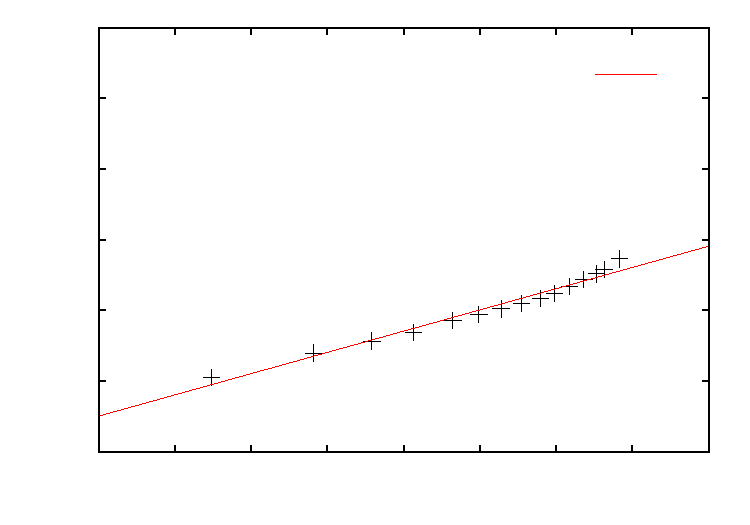
\includegraphics{Diagramme/anodenstromkurve-logarithmisch}}%
    \gplfronttext
  \end{picture}%
\endgroup

\end{figure}


\subsection{Ionisierungsarbeit von Quecksilber}
\label{sec:ionis-von-quecks}

In diesem Versuchsteil wird das Gitter $G_1$ als Beschleunigungsgitter genutzt. Hierbei liegt $G_1$ auf dem selben Potential wie $G_2$. Als Temperatur wird $T = \SI{120}{\celsius}$ gew�hlt, wobei die Betriebsparameter entsprechend 1.2 eingestellt werden. 

Zun�chst wird der Anodenstrom gegen die Beschleunigungsspannung (korrigiert um Thermokontaktspannung) aufgetragen.


Im Diagramm erkennt man einen typischen Knick, dessen Spannungswert der Ionisierungsarbeit in $\si{\eV}$ entspricht. Legt man durch die Punkte vor und nach dem Knick eine Regressionsgerade und bestimmt deren Schnittpunkt, so erh�lt man
\begin{align*}
  E_{\mathrm{Ion.}} = \SI{}{\eV}
\end{align*}
Verglichen mit dem Literaturwert von $E_{\mathrm{Ion.}} = \SI{10,44}{\eV}$ ergibt sich eine relative Abweichung von \%.

Nun wird der Auff�ngerstrom gegen die Beschleunigungsspannung aufgetragen und mittels Oszilloskop (\textit{Picoscope}) die Position der Spannungsspitze ermittelt. Diese liegt bei $U_2 = \SI{13,38}{\volt}$. Korrigiert man um die Thermokontaktspannung, so erh�lt man $U = \SI{}{\volt}$, bzw. 
\begin{align*}
  E_{\mathrm{Ion.}} = \SI{}{\eV}
\end{align*}

\end{document}